\chapter*{Preface}

After defending my PhD thesis in 2020, I swore to take a good break
from the stress of academia, and spent a gap year in Athens, Greece.
This turned out to be the most prolific year of my career. In the absence
of external pressure, I could finally get some research done.

It was during that summer of 2021 that I started designing a new course on
\emph{Blockchain Foundations}. This 56-hour course aimed to answer
three questions:

\begin{enumerate}
  \item What are blockchains?
  \item How do they work?
  \item Why are they secure?
\end{enumerate}

I found that there was already a corpus of works describing the
details of blockchains. However, that literature was not quite what
I was looking for. Some of it was scattered across informal blog posts
and YouTube videos
that explained high-level ideas tailored towards end users or
hobby scientists, and never went down to the mathematical details.
Other writings were \emph{very} precise on the engineering level
--- talking about this or that byte of a packet --- but never explained
the \emph{why} behind the design decisions, and in particular they
were missing security proofs against arbitrary adversaries.
Many of the technical specifications of various cryptocurrencies
fall into this category.
Lastly, a body of works of high quality \emph{does} provide mathematical
proofs and justification
for the \emph{whys}, but these are in the form of scientific papers
that are extremely dense and beyond the reach of even advanced graduate
students, let alone undergraduates dipping their feet on blockchain
science for the first time. I decided it's about time to write a
series of lecture notes on the foundations to accompany the lectures.

As I was designing the course, I trialed it to a group of my computer
science colleagues with no prior blockchain experience:
Giannis Gkoulioumis, Nikolaos Kamarinakis, Apostolos Tzinas.
Over the course of that summer, we spent 52-hours together over notebooks
of notes, discussing the proofs of \emph{bitcoin backbone} and the
construction of Merkle trees. They also solved a series of programming
exercises which I designed to accompany the course and pertained to
creating their own blockchain from scratch, each building their own
full node. Their feedback gave me the opportunity to refine the course
and prepare it for teaching.

% \begin{figure}[h]
%     \centering
%     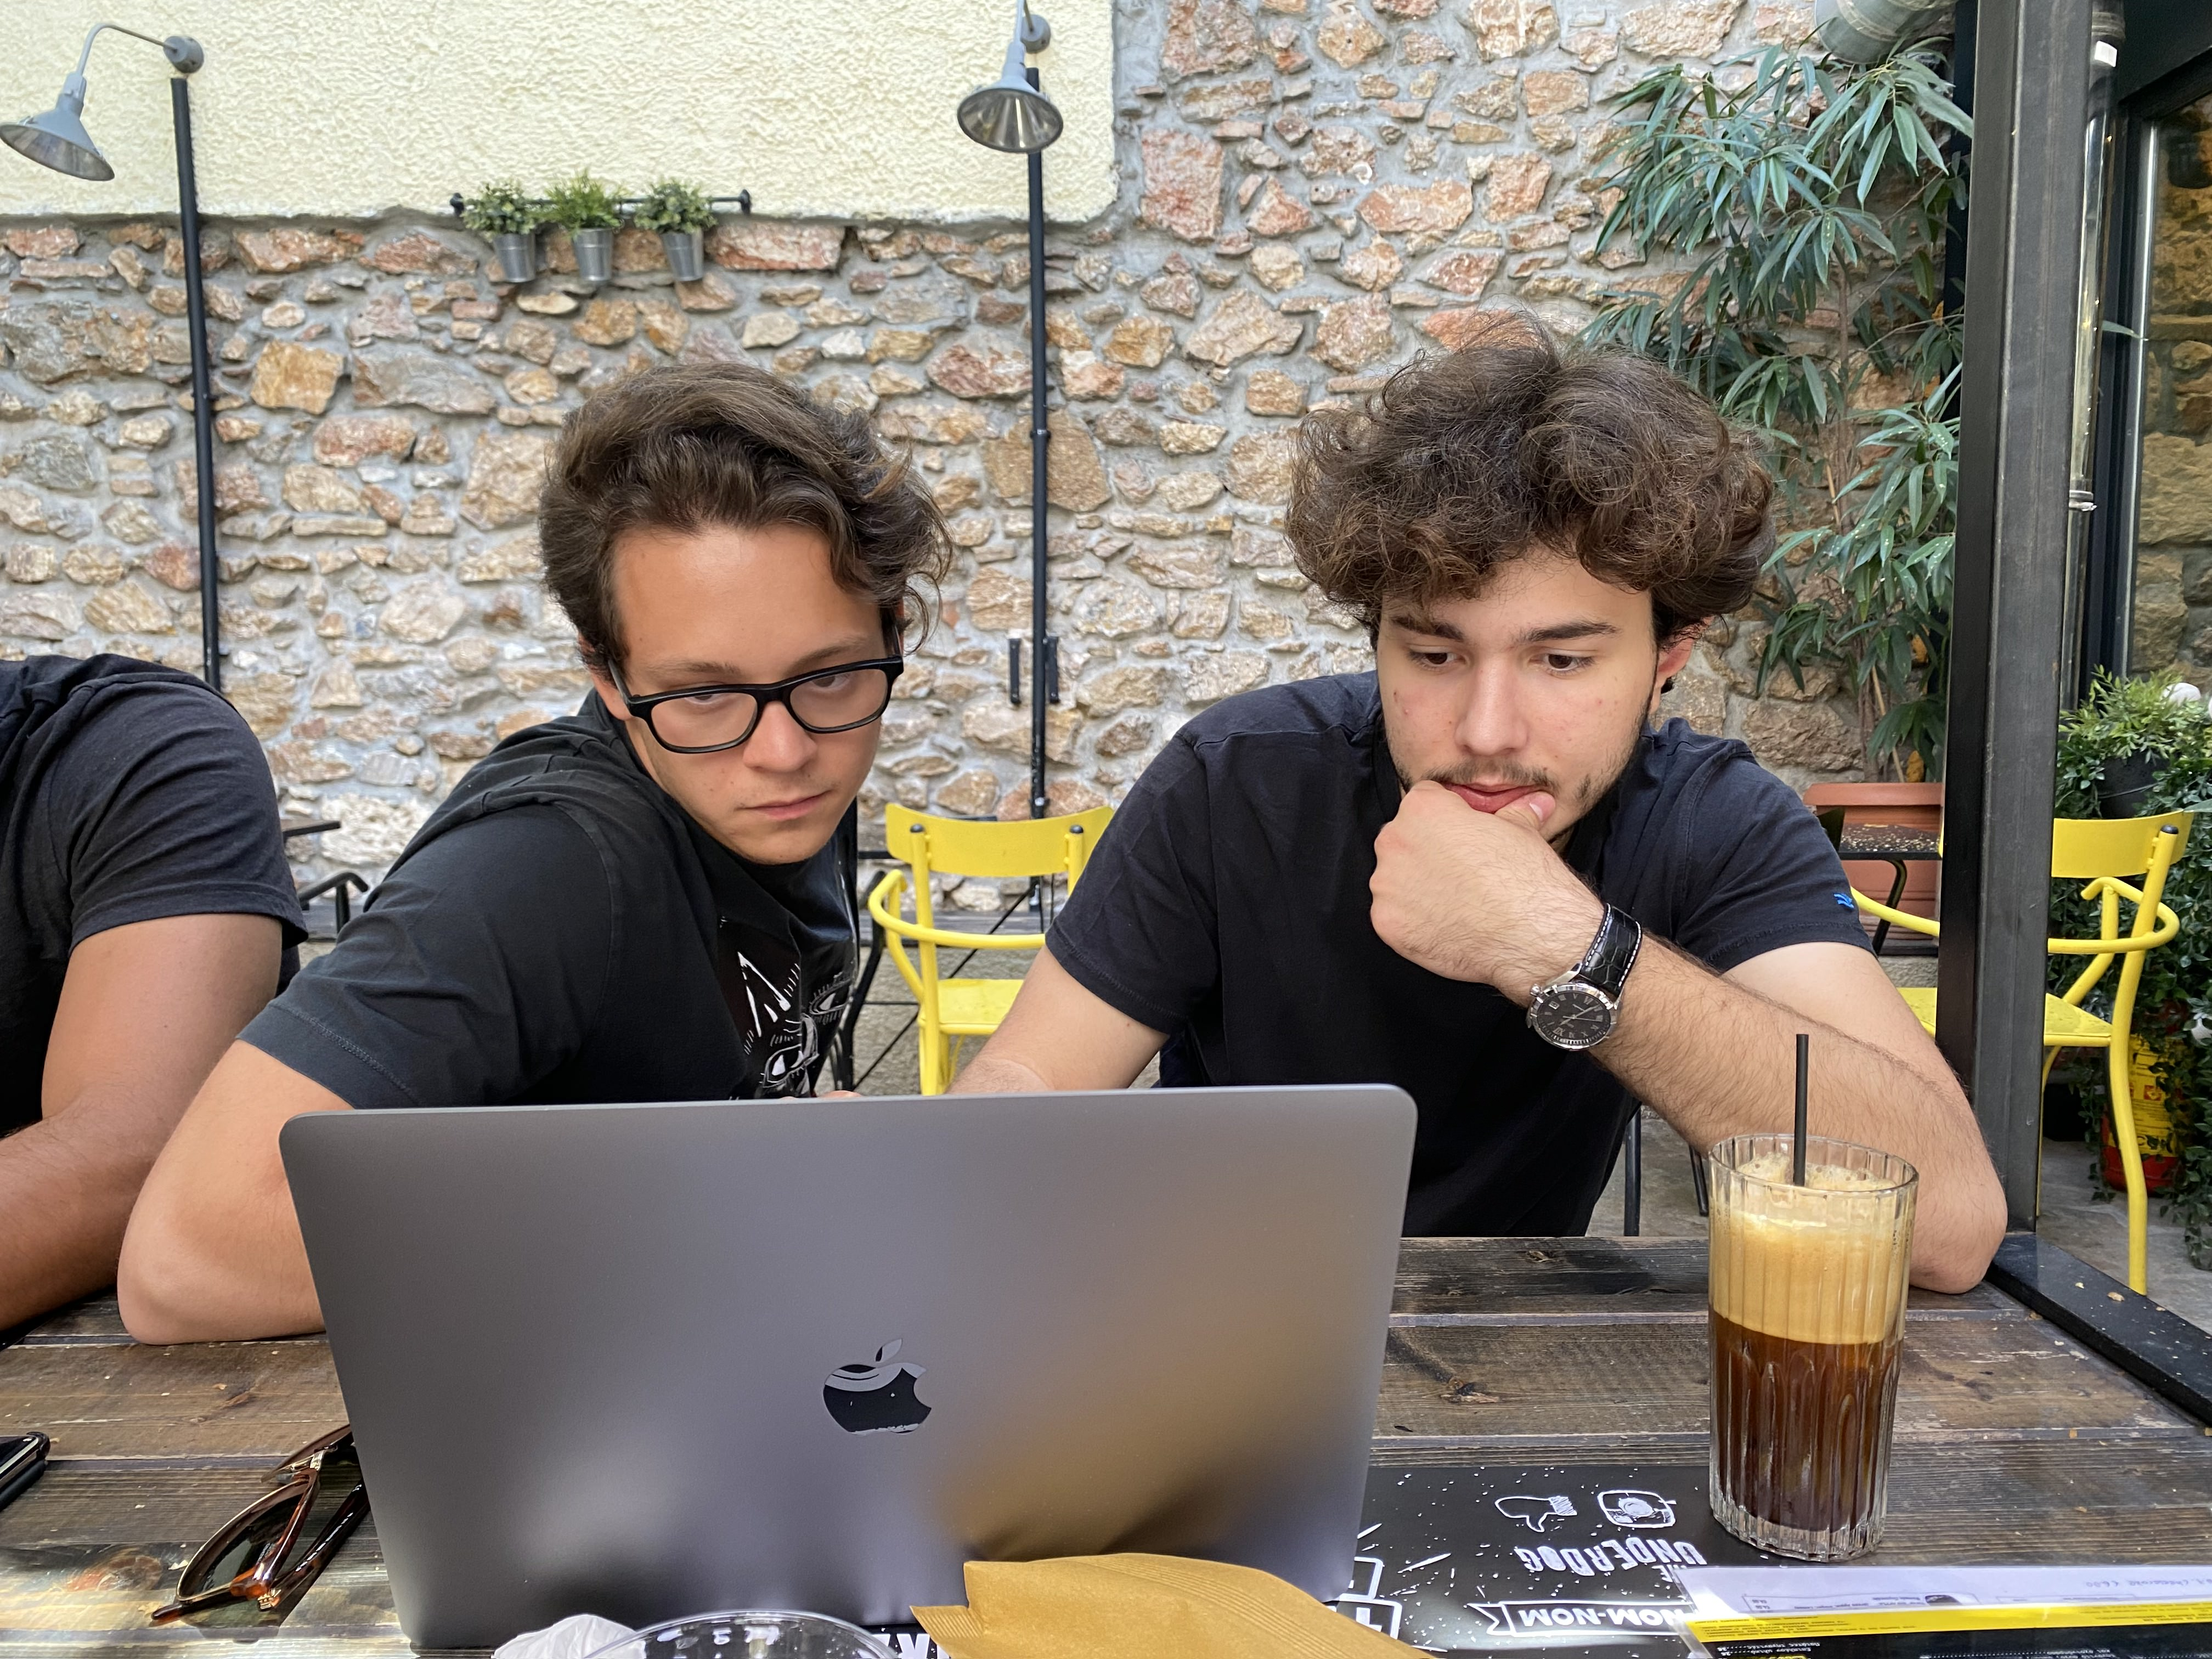
\includegraphics[width=0.6 \columnwidth,keepaspectratio]{figures/k4m4-tzinas.jpg}
%     \caption{Nikolas and Apostolos, two of the students I first taught this course to as a trial,
%     working on the implementation of their \emph{Marabu} node and drinking their
%     \emph{Freddo Espresso} coffee during the Greek summer of 2021 in Athens.}
%     \label{fig.k4m4-tzinas}
% \end{figure}
% 
I had the first opportunity to teach this course --- which I nicknamed
\emph{Marabu}\footnote{The misspelling is intentional, as it makes it easier to Google.}
after the eponymous poem of Nikos Kavvadias --- in an official capacity during the
spring quarter of 2022 at Stanford University. It was a graduate-level course
named EE374 - Blockchain Foundations. While most of the material was
based on my past summer, my co-instructor David Tse and I redesigned
parts of the course to meet the time constraints of the quarter system,
and to include some new material. To our surprise, the course was mostly
attended by undergraduates.
The course was well received,
largerly due to the great work of our first teaching assistants,
Srivatsan Sridhar and Kamilla Nazirkhanova.

At the time, the lecture notes were still
in my handwritten notebooks. As I taught the lectures on the whiteboard,
several students helped out with digitizing the lecture notes to
form the first version of this book. These scribes were
Kaylee Renae George, Kenan Hasanaliyev, Koren Gilbai,
Ben Choi, Stephen Su, Nathaniel Masfen-Yan,
Schwinn Saereesitthipitak, Kachachan Chotitamnavee, Alan Zhang,
Taher Poonawala, Scott Hickmann,
Lyron Co Ting Keh, Sam Liokumovich,
Kaili Wang, Andrej Elez,
Edward Vendrow, Cathy Zhou,
Yifan Yang,
Michael Nath, Coleman Smith,
Solal Afota,
Suppakit Waiwitlikhit, Lora Xie,
Bryan Chiang, Lucas Xia,
% below here are for David's notes, but let's keep their names
Albert Pun, Gordon Chi,
Jack Liu,
Neetish Sharma, Sergio Charles,
Priyanka Mathikshara, and John Guibas.
Even though these notes were later rewritten many times,
I'm deeply grateful to all, because they made the first version happen,
and it would not have started without them.

We repeated this course during winter quarter of 2023.
There, our teaching assistants were Kenan Hasanaliyev
and Scott Hickmann who further helped refine the course material and notes.

This book is the result of assembling those lecture notes into a
more organized format. We want the advanced undergraduate or beginning
graduate student to be able to comfortably read it. The prerequisites
are a basic understanding of probabilities; an expert level of programming
knowledge, ideally with some network programming experience; some exposure
to computer science through an introductory algorithms or computability
course, and familiarity with computational reductions;
and, of course, the always elusive \emph{mathematical maturity}.

This book does not talk about Bitcoin or Ethereum. It doesn't speak
about the particularities of these implementations, such as how Bitcoin
encodes addresses, or how Ethereum's particular programming language works.
Instead, we go back to the foundations to understand the basic components
that make a blockchain from first principles. The principles that we explore
apply to most blockchain systems, and even decentralized ledger technology
systems that are not based on a blockchain \emph{per se}. The goal is to learn
how to argue about the security of these systems by walking through the
components of a simple UTXO proof-of-work blockchain design first. The
same design principles apply when designing more complicated systems such
as proof-of-stake blockchains. Upon completing this book, the reader will
know what blockchains are, how they work, and why they are secure. They
will also have developed the tools and background necessary to argue about
the security of more complex protocols.
